% Options for packages loaded elsewhere
\PassOptionsToPackage{unicode}{hyperref}
\PassOptionsToPackage{hyphens}{url}
\documentclass[
 12pt,
 letterpaper,
]{article}
\usepackage{xcolor}
\usepackage{amsmath,amssymb}
\usepackage{listings}
\usepackage{pgfplots}
\pgfplotsset{compat=1.18}
\usepgfplotslibrary{statistics}
\usepackage{float}
\usepackage{placeins}
\usepackage[left=3cm,right=2.5cm,top=2.5cm,bottom=2.5cm]{geometry}
\usepackage{setspace}
\setcounter{secnumdepth}{-\maxdimen} % remove section numbering
\usepackage{iftex}
\ifPDFTeX
  \usepackage[T1]{fontenc}
  \usepackage[utf8]{inputenc}
  \usepackage{textcomp} % provide euro and other symbols
\else % if luatex or xetex
  \usepackage{unicode-math} % this also loads fontspec
  \defaultfontfeatures{Scale=MatchLowercase}
  \defaultfontfeatures[\rmfamily]{Ligatures=TeX,Scale=1}
\fi
\usepackage{lmodern}
\ifPDFTeX\else
  % xetex/luatex font selection
\fi
% Use upquote if available, for straight quotes in verbatim environments
\IfFileExists{upquote.sty}{\usepackage{upquote}}{}
\IfFileExists{microtype.sty}{% use microtype if available
  \usepackage[nopatch=footnote]{microtype}
  \UseMicrotypeSet[protrusion]{basicmath} % disable protrusion for tt fonts
}{}
\makeatletter
\@ifundefined{KOMAClassName}{% if non-KOMA class
  \IfFileExists{parskip.sty}{%
    \usepackage{parskip}
  }{% else
    \setlength{\parindent}{0pt}
    \setlength{\parskip}{6pt plus 2pt minus 1pt}}
}{% if KOMA class
  \KOMAoptions{parskip=half}}
\makeatother
\setlength{\parindent}{0pt}
\setlength{\parskip}{0.4em}
\onehalfspacing
\setlength{\emergencystretch}{3em} % prevent overfull lines
\providecommand{\tightlist}{%
  \setlength{\itemsep}{0pt}\setlength{\parskip}{0pt}}
\usepackage{bookmark}
\IfFileExists{xurl.sty}{\usepackage{xurl}}{} % add URL line breaks if available
\urlstyle{same}
\hypersetup{
  hidelinks,
  pdfcreator={LaTeX via pandoc}}

\lstdefinestyle{pseudocodigo}{
  backgroundcolor=\color{gray!15},
  basicstyle=\ttfamily\small,
  frame=single,
  framerule=0pt,
  xleftmargin=0.5em,
  xrightmargin=0.5em,
  aboveskip=1em,
  belowskip=1em,
  showstringspaces=false,
  inputencoding=utf8,
  literate=
    {á}{{\'a}}1 {é}{{\'e}}1 {í}{{\'i}}1 {ó}{{\'o}}1 {ú}{{\'u}}1
    {Á}{{\'A}}1 {É}{{\'E}}1 {Í}{{\'I}}1 {Ó}{{\'O}}1 {Ú}{{\'U}}1
    {ñ}{{\~n}}1 {Ñ}{{\~N}}1
    {ü}{{\"u}}1 {Ü}{{\"U}}1
    {¿}{{?`}}1 {¡}{{!`}}1
}

\author{}
\date{}

\begin{document}

\textbf{Análisis y optimización matemática de modelos con Naive Bayes en
sistemas de almacenamiento para el proyecto Conductome.}

\renewcommand{\contentsname}{Índice}
\tableofcontents
\newpage

\section{Capítulo 1. Introducción}\label{capuxedtulo-1.-introducciuxf3n}

\subsection{\texorpdfstring{\textbf{1 Contexto del proyecto Conductoma y
Project42.}}{1 Contexto del proyecto Conductoma y Project42.}}\label{contexto-del-proyecto-conductoma-y-project42.}

La idea principal del proyecto Conductome y de Project42 es,
considerando que todo lo que nos rodea está ahí por una cadena de
decisiones elegidas por todos los habitantes de este planeta, busca
enfocarse en los problemas que enfrenta la humanidad actualmente como
obesidad, hipertensión y diferentes enfermedades crónicas. Mediante un
proceso de inferencia estadística, se busca entender mejor cuales son
los motivos por los que estos problemas ocurren, desde el punto de vista
de la conducta humana.

Una de las claves para la construcción del conductome es contemplar
datos que trascienden las disciplinas, mismas que a primera vista
pudieran no tener mucha relación, al considerarse como conjunto puedan
revelar patrones de comportamiento que deriven en alguno de los
problemas mencionados anteriormente.

Sabemos que algunos factores de riesgo importantes para la obesidad van
desde lo genético hasta lo económico y político. Conductome busca
aportar factores considerando la conducta humana, comportamientos poco
saludables durante largos periodos. Comportamientos que a su vez están
afectados por nuestro entorno, ambiente obesogénico en el que vivimos y
por la percepción del mundo y de nosotros mismos.

Desde el punto de vista matemático, se puede abordar el problema usando
inferencia estadística sobre los datos disponibles. Consideramos un
conjunto de variables que describen la conducta y características
individuales de una población y fijamos una cierta clase objetivo
usualmente asociada a un padecimiento de salud como diabetes o
hipertensión.

Project42 busca saber si una selección de variables explica ``bien'' o
``mal'' a la clase dada, mediante el uso de métricas como el Epsilon y
Score, calculados a partir de probabilidades condicionales asociadas a
cada categoría se puede concluir sin interpretación que tan bien se
explica la clase (o la no clase).

Los detalles formales del modelo, así como de los métodos de estimación
y métricas usadas para evaluar la capacidad explicativa de las
variables, se desarrollarán con más detalle en capítulos posteriores.

La parte de la implementación computacional puede llegar a ser compleja
en estos modelos como se verá más adelante. Sin embargo parte del
objetivo de este trabajo es analizar y optimizar desde la recolección de
datos hasta el procesamiento de éstos, con el fin de lograr calcular las
métricas Epsilon y Score en un tiempo mucho menor al que actualmente se
puede conseguir.

\subsection{1.2 Estructura de la tesis.}\label{estructura-de-la-tesis.}

El trabajo aquí presentado se organiza de la siguiente manera. En el
capítulo 1 se trata de introducir al lector al proyecto Conductome así
como a Project42, su contexto e idea general.

En el capítulo 2 se ven los conceptos matemáticos necesarios para el
completo entendimiento de los proyectos, incluyendo teorema de Bayes,
discretización de variables y la definición de métricas explicativas
usadas en Project42 como el epsilon y score de una categoría, entre
otros.

En el capítulo 3 se formaliza el modelo en particular usado en
Project42, se formalizan las poblaciones utilizadas, las variables
objetivo, variables dependientes e independientes.

En el capítulo 4 se analiza la actual implementación de este modelo en
la plataforma en línea y se proponen diferentes soluciones tanto en la
recuperación de los datos, así como el manejo y flujo de datos para la
construcción de las métricas epsilon y score.

En el capítulo 5 vemos los resultados obtenidos de la implementación de
las soluciones propuestas. Evaluando y analizando resultados en el
performance reales para poder concluir cuál es la solución más eficiente
estadísticamente.

En el capítulo 6 el trabajo concluye con una discusión de los
resultados, posibles mejoras y limitaciones de la versión actual y
propuestas a futuro.

\subsection{1.3 Problema matemático y
computacional.}\label{problema-matemuxe1tico-y-computacional.}

\textbf{Detallar problema matemático, calculos de probabilidades, etc.}

Podremos notar que generar las métricas Epsilon y Score, usadas para
evaluar que tan bien explican las diferentes variables y sus categorías
una clase dada, requiere del cálculo repetido de probabilidades
condicionales.

La antigua implementación de Project42 hacía este proceso
computacionalmente costoso, lo cual limitaba la exploración eficiente de
diferentes variables para explicar alguna clase dada, pues los tiempos a
esperar para obtener las métricas podía rebasar el minuto de espera,
dependiendo de la cantidad de variables a consultar.

\subsection{1.4 Objetivos.}\label{objetivos.}

Tenemos como objetivos principales, explicar la teoría detrás de los
proyectos Conductome y Project42, entender el porqué las métricas
Epsilon y Score funcionan. Posteriormente pasar a analizar y optimizar
el proceso de obtención de estas métricas, mediante la reformulación del
flujo de datos, representación de éstos y su procesamiento con el fin de
reducir el costo computacional sin alterar ninguna de las propiedades
del modelo original.

Objetivos específicos:

1.- Formular matemáticamente el modelo estadístico usado en Project42.

2.- Analizar la complejidad temporal y espacial del algoritmo que
calcula epsilon y score dados un conjunto de variables y una clase.

3.- Proponer una implementación en pseudocódigo del algoritmo encargado
de calcular las métricas Epsilon y Score.

4.- Comparar teórica y empíricamente el desempeño de los diferentes
algoritmos propuestos, así como de diferentes filosofías de diseño para
la recuperación de los datos usados para el cálculo de Epsilon y Score.

\section{Capítulo 2. Preliminares
Matemáticos.}\label{capuxedtulo-2.-preliminares-matemuxe1ticos.}

En este capítulo se presentan los fundamentos matemáticos necesarios
para el desarrollo del trabajo. Se asume que el lector cuenta con
conocimientos básicos de probabilidad, estadística y análisis de
algoritmos, ya que se profundizará únicamente los conceptos directamente
relacionados con los proyectos Conductome y Project42.

Empezando con conceptos como minería de datos, con el fin de
contextualizar el uso de modelos estadísticos en conjuntos de datos con
muchas variables (multidimensionales) . Después se ven conceptos básicos
de probabilidad y estadística que fundamentan los modelos de
clasificación usando las métricas Epsilon y Score.

Se introduce el teorema de Bayes así como del clasificador basado en
éste Naive Bayes, el cual es fundamental para la construcción del
sistema usado en Project42. Se analizan sus variantes para casos
continuos y limitantes en términos de clasificación.

Se definen formalmente las métricas Epsilon y Score anteriormente
mencionadas y se analiza su desempeño al usarse para la creación de un
clasificador binario.

Finalmente se desarrollan algunos criterios para la evaluación de
modelos, es decir, buscamos formas para concluir si un modelo es
``bueno'' para clasificar independientemente de sus datos. Así como
nociones de complejidad algorítmica, útiles para determinar el costo
computacional de los algoritmos posteriormente propuestos.

\subsection{2.1 Minería de datos.}\label{mineruxeda-de-datos.}

Podemos definir a la minería de datos como una rama del análisis de
datos que se encarga de encontrar patrones ``ocultos''. Con ayuda del
poder de cómputo actual la minería de datos es capaz de transformar un
conjunto de datos en conocimiento práctico, el cual puede ser utilizado
para determinar conductas de consumo, o consecuencias por una toma de
decisiones empresariales, lo cual es de extrema utilidad para las
empresas privadas y que puedan aumentar sus márgenes de beneficio.

Una gran diferencia entre la minería de datos y otros métodos de
análisis más clásicos, son la cantidad de variables y observaciones
utilizadas para obtener conclusiones. Mientras que un acercamiento por
análisis más clásico requiere de unos supuestos bien definidos y un
número reducido de variables, en la minería de datos usualmente se
trabaja con bases de datos con una gran cantidad de variables (cientos o
incluso miles) donde no siempre se pueden garantizar supuestos como la
independencia.

En el caso de Project42 y Conductome, se usa la minería de datos para
entender mejor el alto porcentaje de personas con enfermedades
cardiovasculares como obesidad e hipertensión en México.

\subsection{2.2 Conceptos básicos.}\label{conceptos-buxe1sicos.}

\textbf{Axiomas de probabilidad.}

Recordemos que un axioma es una proposición que se toma como verdadera y
sobre el cual se fundamentan diferentes resultados. Decimos que $\mathbb{P} \colon \Omega \to [0, 1]$ es una
función de probabilidad si cumple con los siguientes axiomas.

\begin{enumerate}
\def\labelenumi{\arabic{enumi}.}
\item
  $\mathbb{P}(A) \geq 0$, para todo $A \subseteq \Omega$
\item
  $\mathbb{P}(\Omega) = 1$
\item
  La probabilidad de la union numerable de subconjuntos ajenos dos a dos
  es igual a la suma de las probabilidades individuales. A esta
  propiedad se le llama aditividad. Esto es, si $A_1, A_2, \ldots$ son subconjuntos de $\Omega$ tales que
   $A_i \cap A_j = \emptyset$ para todo $i \neq j$, entonces:
  \[
  \mathbb{P}\left(\bigcup_{i=1}^{\infty} A_i\right) = \sum_{i=1}^{\infty} \mathbb{P}(A_i)
  \]
\end{enumerate} 
\medskip

\noindent\textbf{Sigma-álgebra.}

La idea de una sigma-álgebra es un conjunto que agrupa a todos los
eventos de un mismo experimento aleatorio. Aunque a primera vista estos
conjuntos parecen bastante abstractos, son extremadamente útiles para
los posteriores cálculos de probabilidades.

Sea $\Omega$ un conjunto, decimos que $F$ es una sigma-álgebra de subconjuntos de $\Omega$ si se cumplen las siguientes 
propiedades:

\begin{enumerate}
\def\labelenumi{\arabic{enumi}.}
\item
  $\Omega \in F$
\item
  Si $A \in F$ entonces $\Omega \setminus A \in F$ (el complemento pertenece a $\Omega$)
\item
  Si $A_1, A_2, \ldots \in F$ entonces la unión numerable pertenece a $F$
\end{enumerate}

A los elementos de F se les llama eventos.

Un par de sigma-álgebras inmediatas son $\{\emptyset, \Omega\}$ y el conjunto potencia de Omega $\mathcal{P}(\Omega)$.

Con este par de conceptos podemos dar paso a la definición de un espacio
de probabilidad para un experimento aleatorio.

Un espacio de probabilidad es una terna $(\Omega, F, \mathbb{P})$ donde $\Omega$ es un
conjunto, $F$ es una sigma-álgebra de subconjuntos de $\Omega$ y $\mathbb{P}$ es una función
de probabilidad definida sobre F.

\textbf{Sigma álgebra de Borel.}

\textbf{Probabilidad condicional.}

La probabilidad condicional es un concepto sencillo pero que es muy útil
para el cálculo de probabilidades, pues ayuda a reducir ciertas
probabilidades a expresiones más sencillas.

Sean $A$ y $B$ dos eventos tal que $\mathbb{P}(B) > 0$.

Definimos la probabilidad condicional del evento $A$ dado $B$, $\mathbb{P}(A\mid B)$,
como:

\[
\mathbb{P}(A\mid B) = \dfrac{\mathbb{P}(A\cap B)}{\mathbb{P}(B)}
\]

La idea intuitiva de la probabilidad condicional es considerar un evento
B que ya ha ocurrido y ver cómo esta información adicional influye sobre
la probabilidad de A.

Uno puede considerar que usar la probabilidad condicional $\mathbb{P}(A\mid B)$
es como reducir el espacio muestral $\Omega$ al evento $B$, de tal forma que
cualquier evento que ocurra fuera de B tiene probabilidad condicional
cero.

\textbf{Teorema de Bayes.}

El teorema de Bayes es uno de esos resultados fundamentales en la teoría
de la probabilidad, ya que, permite calcular probabilidades
condicionales en términos de la probabilidad condicional invertida, es
decir, se pueden calcular probabilidades condicionales a partir de la
observación de evidencia.

En el contexto de Project42, se usa el teorema de Bayes para calcular
que tan probable es que una persona pertenezca a una clase de interés
dado un conjunto de variables explicativas, probabilidad que
eventualmente será útil para la construcción de epsilon y score.

Sean $A$ y $B$ dos eventos tales que $\mathbb{P}(B) > 0$. Entonces:

\[
\mathbb{P}(A \mid B) = \dfrac{\mathbb{P}(B \mid A)\,\mathbb{P}(A)}{\mathbb{P}(B)}
\]

\textbf{Demostración:}

Por definición de probabilidad condicional, tenemos que:

\[
\mathbb{P}(A \mid B) = \dfrac{\mathbb{P}(A \cap B)}{\mathbb{P}(B)}
\]

Y que
\[
\mathbb{P}(B \mid A) = \dfrac{\mathbb{P}(B \cap A)}{\mathbb{P}(A)} = \dfrac{\mathbb{P}(A \cap B)}{\mathbb{P}(A)}
\]

Despejando $\mathbb{P}(A \cap B)$ de esta última expresión tenemos:

\[
\mathbb{P}(A \cap B) = \mathbb{P}(B \mid A)\,\mathbb{P}(A)
\]

Y sustituyendo en la primera expresión:

\[
\mathbb{P}(A \mid B) = \dfrac{\mathbb{P}(B \mid A)\,\mathbb{P}(A)}{\mathbb{P}(B)}
\]

En esta expresión, es común encontrar que a los términos se les denomine
de la siguiente forma:

$\mathbb{P}(A)$ la probabilidad a priori.

$\mathbb{P}(A \mid B)$ la probabilidad a posterior.

$\mathbb{P}(B \mid A)$ se le denomina verosimilitud.

Con este resultado podemos considerar que la probabilidad de una
hipótesis se actualiza al agregarse nueva evidencia. En el caso de
Project42, la hipotesis corresponde con la pertenencia de un individuo a
cierta clase (individuo con diabetes, obesidad, sobrepeso, etc), y la
evidencia agregada son los valores observados en las diferentes
variables explicativas (edad, actividad física, alimentación, etc).

\textbf{Independencia de eventos.}

El concepto de independencia de eventos representa la idea de que la ocurrencia de un evento no afecta 
la probabilidad de ocurrencia de otro evento. Este concepto ayuda a simplificar el cálculo de algunas 
probabilidades.

Definición.

Sean $A$ y $B$ dos eventos, decimos que $A$ y $B$ son independientes si se cumple la igualdad:
$$\mathbb{P}(A \cap B) = \mathbb{P}(A)\,\mathbb{P}(B).$$

Si a esta definición le agregamos la hipotesis de que $\mathbb{P}(B) > 0$, entonces:

$$\mathbb{P}(A \mid B) = \mathbb{P}(A).$$

Esto es, que la ocurrencia de $B$ no afecta la probabilidad del evento $A$.

\textbf{Variable aleatoria discreta.}

Sea $(\Omega, F, \mathbb{P})$ un espacio de probabilidad. Definimos una variable
aleatoria $X$ como una transformación del espacio de resultados $\Omega$ al
conjunto de números reales, esto es,

\[
X:\Omega \to \mathbb{R}
\]
tal que para cualquier elemento de la sigma álgebra de Borel $B$, la
imagen inversa $X^{-1}(B) \in F$.

(Notación: $(X \in A) = \{w \in \Omega \mid X(w) \in A\}$, que en otras
palabras es la imagen inversa de $A$ bajo $X$. De igual manera con $(X \in (a,
b)) = \{w \in \Omega \mid a < X(w) < b\}$.)

Una observación importante es que cuando $\Omega$ es a lo mas numerable y $F =
\mathbb{P}(\Omega)$, entonces cualquier función $X:\Omega \to \mathbb{R}$ cumple con la
definición de ser variable aleatoria.

Detrás de esta definición que puede parecer muy abstracta, podemos
considerar a las variables aleatorias como una pregunta o medición a los
resultados de un experimento aleatorio y cuya respuesta es un número
real. Para ilustrar la idea veamos un par de ejemplos.

\textbf{Ejemplo 1.}

Consideremos el experimento aleatorio de un volado, esto es, lanzar una
moneda equilibrada al aire y ver cuál es la cara que está mirando hacía
arriba.

Denotemos por ``Cara'' y ``Cruz'' a los dos diferentes lados de la
moneda, con esto construimos el espacio muestral $\Omega = \{\text{Cara},
\text{Cruz}\}$ y la sigma álgebra $F = \mathbb{P}(\Omega)$, definimos a la función $X$ de la
siguiente manera:

\[
X:F \to \mathbb{R}, \qquad X(\text{Cruz}) = 1, \quad X(\text{Cara}) = 0.
\]

Por la observación de arriba se sigue que X cumple con ser variable
aleatoria. Con esto podemos empezar a calcular algunas probabilidades.

\begin{align*}
\mathbb{P}(X = 1)
&= \mathbb{P}(\{w \in \Omega \mid X(w) = 1\})
= \mathbb{P}(\{\text{Cruz}\})
= \tfrac{1}{2}, \\
\mathbb{P}(X \in [1,2))
&= \mathbb{P}(\{w \in \Omega \mid 1 \le X(w) < 2\})
= \mathbb{P}(\{\text{Cruz}\})
= \tfrac{1}{2}, \\
\mathbb{P}(X \in (10,20))
&= \mathbb{P}(\{w \in \Omega \mid 10 < X(w) < 20\})
= \mathbb{P}(\emptyset)
= 0, \\
\mathbb{P}(X < -1)
&= \mathbb{P}(\{w \in \Omega \mid X(w) < -1\})
= \mathbb{P}(\emptyset)
= 0, \\
\mathbb{P}(X > 0)
&= \mathbb{P}(\{w \in \Omega \mid 0 < X(w)\})
= \mathbb{P}(\{\text{Cruz},\text{Cara}\})
= 1.
\end{align*}

\textbf{Ejemplo 2.}

Consideremos el experimento aleatorio de lanzar dos dados equilibrados.
Aquí nuestro espacio muestral queda definido por pares ordenados (a,b)
de la siguiente manera:

\[
\Omega = \{1,2,3,4,5,6\} \times \{1,2,3,4,5,6\}
= \{(a,b) \mid a,b \in \{1,2,3,4,5,6\}\}.
\]

La sigma-álgebra de $\Omega$ es $F = \mathbb{P}(\Omega)$, la potencia de $\Omega$.

Y la función de probabilidad considera dos dados justos y la definimos
como
\[
\mathbb{P}(\{(a,b)\}) = \tfrac{1}{36}, \qquad \forall (a,b) \in \Omega.
\]

Definamos la variable aleatoria que se fije en la suma de los dados. Sea
\[
S: \Omega \to \mathbb{R}, \qquad S((a,b)) = a+b.
\]

Con esto, podemos calcular algunas probabilidades:
\begin{align*}
\mathbb{P}(S = 7)
&= \mathbb{P}(\{(a,b) \in \Omega \mid a+b=7\}) \\
&= \mathbb{P}(\{(1,6),(2,5),(3,4),(4,3),(5,2),(6,1)\}) \\
&= \tfrac{6}{36} = \tfrac{1}{6}.
\end{align*}
Este último paso se obtiene por aditividad de $\mathbb{P}$.

A pesar del nombre, una variable aleatoria no es variable ni aleatoria,
pero el nombre se justifica al considerar que los diferentes resultados
de un experimento aleatorio son los diferentes números reales x que la
función X puede tomar.

Espacio de probabilidad discreto.

Sea $(\Omega,F,\mathbb{P})$ un espacio de probabilidad, donde $\Omega$ es un conjunto finito o
numerable de resultados. $F$ es la sigma-álgebra de subconjuntos de $\Omega$
y $\mathbb{P}$ es una función de probabilidad sobre $F$.

En el contexto de este trabajo se considerarán únicamente espacios de
probabilidad discretos. \textbf{** Investigar por qué es importante que
NB funciona mejor con espacios discretos.}

\textbf{Función de probabilidad.}

Definición.

Sea $X$ una variable aleatoria discreta con valores posibles $x_1, x_2, \ldots$ Definimos la función de 
probabilidad de $X$, denotada por $f(x): \mathbb{R} \to \mathbb{R}$ como:
\[
f(x)=
\begin{cases}
\mathbb{P}(X = x), & \text{si } x = x_1, x_2, \ldots, \\
0, & \text{en otro caso.}
\end{cases}
\]

\textbf{Esperanza.}

Definición.

Sea $X$ una variable aleatoria discreta con función de probabilidad $f$. Definimos la esperanza de $X$ como:
$$\mathbb{E}[X] = \sum_{x} x\,f(x)$$

Esto suponiendo que la serie es absolutamente convergente, es decir, cuando la suma de los valores absolutos 
es convergente.

Por otro lado, si $X$ es una variable aleatoria continua con función de densidad $f$, entonces la esperanza de $X$ se define como:
$$\mathbb{E}[X] = \int_{-\infty}^{\infty} x\,f(x)\,dx$$

Donde ahora suponemos que la integral es absolutamente convergente, es decir, que la integral de los 
valores absolutos es convergente.

La esperanza de una variable aleatoria se puede interpretar como el promedio ponderado de los posibles 
valores que puede tomar la variable, donde los pesos son las probabilidades de cada valor. A la esperanza 
también se le conoce como valor esperado o valor promedio. 

\textbf{Varianza.}

Definición.

Sea $X$ una variable aleatoria discreta con esperanza $\mathbb{E}[X]$ y función de probabilidad $f$. 
Definimos la varianza de $X$ como:
$$\text{Var}(X) = \sum_{x} (x - \mathbb{E}[X])^2\,f(x)$$

Esto suponiendo que la serie es convergente.

Por otro lado, si $X$ es una variable aleatoria continua con función de densidad $f$ y esperanza 
$\mathbb{E}[X]$, entonces la varianza de $X$ se define como:
$$\text{Var}(X) = \int_{-\infty}^{\infty} (x - \mathbb{E}[X])^2\,f(x)\,dx$$

cuando la integral es convergente.

La varianza de una variable aleatoria se puede interpretar como una medida de dispersión de los posibles 
valores que puede tomar la variable, es decir, mide que tan alejados están los valores de la variable respecto 
a su esperanza. A la raiz cuadrada de la varianza $\sqrt{\text{Var}(X)}$ se le conoce como 
desviación estándar.

\textbf{Función generadora de momentos.}

Esta es otra función útil que se calcula sobre algunas variables aleatorias y en ésta podemos incluir 
tanto variables discretas como continuas.

Definición.

Sea $X$ una variable aleatoria, definimos $M(t)$ la función generadora de momentos de $X$ como:
$$M(t) = \mathbb{E}[e^{tX}]$$

Para valores de $t$ para los cuales esta esperanza es finita.

\textbf{Odds ratio.}

Definición:

Sean $X$ y $C$ dos vectores aleatorios.

Le llamamos la proporción posterior de $C_1$ respecto a $C_2$ a la proporción
de densidad posterior $\mathbb{P}(C \mid X)$ evaluada en los puntos $C_1$ y $C_2$.

Esto es:

\[
\dfrac{\mathbb{P}(C_1 \mid X)}{\mathbb{P}(C_2 \mid X)}
\]

Notemos que al aplicarse el teorema de Bayes a esta expresión se puede
reducir a lo siguiente:

\begin{align*}
\dfrac{\mathbb{P}(C_1\mid X)}{\mathbb{P}(C_2\mid X)}
&= \dfrac{\dfrac{\mathbb{P}(C_1)\,\mathbb{P}(X\mid C_1)}{\mathbb{P}(X)}}{\dfrac{\mathbb{P}(C_2)\,\mathbb{P}(X\mid C_2)}{\mathbb{P}(X)}} \\
&= \dfrac{\mathbb{P}(C_1)\,\mathbb{P}(X\mid C_1)}{\mathbb{P}(C_2)\,\mathbb{P}(X\mid C_2)}.
\end{align*}

Usualmente esta expresión es utilizada con parámetros $C_1$ y $C_2$ discretos,
tales que $C_2$ es el complemento de $C_1$.

\section{Capítulo 3. Modelado matemático de
Project42.}\label{capuxedtulo-3.-modelado-matemuxe1tico-de-project42.}

En este capítulo buscamos formalizar matemáticamente el sistema
implementado en la plataforma de Project42. Más específicamente queremos
formalizar los conjuntos de datos, el modelo estadístico utilizado y el
criterio usado para evaluar la capacidad explicativa de las variables
usadas.

En Project42 se cuenta con cuatro poblaciones, cada una de las cuales
cuenta con diferentes características o variables, todas orientadas a
encontrar patrones en los padecimientos de salud, sin embargo todas se
trataron para compartir una estructura de datos similar, con el objetivo
de que la creación de modelos sea independiente del origen de los datos.
Con este enfoque, el proyecto puede interpretarse como una plataforma
para el análisis explicativo de variables mediante clasificación
bayesiana.

Sin embargo, en este capítulo nos enfocaremos en la formalización de los
conjuntos de datos utilizados por Project42, asi como de la clase
objetivo y el conjunto de variables independientes (o explicativas) y a
partir de estos elementos calcular y analizar las métricas epsilon y
score.

\subsection{3.1 Naive Bayes.}\label{naive-bayes.}

Naive Bayes es un algoritmo de clasificación que como su nombre lo
indica está basado en el teorema de Bayes, en otras palabras, Naive
Bayes es una función $NB: \Omega \to \mathbb{R}$, tal que $NB(X = x)$ nos
da la clase más probable a la que pertenece el vector aleatorio $X = x$.

El término Naive (ingenuo) viene de que el algoritmo asume independencia
entre las diferentes entradas del vector X = x.

Consideremos una muestra aleatoria $M$, $n$ variables aleatorias $X_1, \ldots,
X_n$ y una variable objetivo $C$ con $k$ diferentes valores, $C_1, \ldots, C_k$.
Entonces la idea de Naive Bayes es preguntarse, dada una observación $x_i$
$= (x_{1i}, x_{2i}, \ldots, x_{ni})$, cuál es la probabilidad de que $x_i$ pertenezca
a la clase $C_j$ para algún $j \le k$. De esta manera Naive Bayes
``predice'' que la observación $x_i$ pertenece a la clase que maximiza la
siguiente probabilidad:

\[
\mathbb{P}(C = C_j \mid x_i) = \dfrac{\mathbb{P}(C = C_j)\,\mathbb{P}(x_i \mid C = C_j)}{\mathbb{P}(x_i)}
\]
(Teo. Bayes).

Sin embargo, calcular las verosimilitudes ($\mathbb{P}(x_i \mid C = C_j)$)
puede ser complejo y en la práctica algo casi imposible. Se puede dar el
caso en que un valor en específico $x_i = (X_1 = x_{1i}, X_2 = x_{2i}, \ldots, X_n
= x_{ni})$ sea un valor que no exista en el conjunto de datos o bien el
número de observaciones en éste no sea suficiente para estimar con un
buen nivel de confianza la probabilidad de pertenencia a la clase.

Aquí es donde el supuesto de independencia entre las diferentes entradas
de $X = (X_1, X_2, \ldots, X_n)$ entra en juego. Al considerar considerar
independencia, podemos considerar lo siguiente:

Sean $A$ y $B$ dos eventos condicionalmente independientes dado un evento $C$,
si:

\[
\mathbb{P}(A \cap B \mid C) = \mathbb{P}(A \mid C)\,\mathbb{P}(B \mid C)
\]

Entonces, la verosimilitud $\mathbb{P}(x_i \mid C = C_j)$ se puede calcular de
la siguiente manera:

\begin{align*}
\mathbb{P}(x_i \mid C = C_j)
&= \mathbb{P}(X_1 = x_{1i} \cap X_2 = x_{2i} \cap \ldots \cap X_n = x_{ni} \mid C = C_j) \\
&= \mathbb{P}(X_1 = x_{1i} \mid C = C_j) \cdot \ldots \cdot \mathbb{P}(X_n = x_{ni} \mid C = C_j),
\end{align*}
con $i = 1, 2, \ldots, n$.

Por lo tanto, la probabilidad a posterior queda de la siguiente manera:

\[
\mathbb{P}(C = C_j \mid x_i) = \dfrac{\mathbb{P}(C = C_j) \cdot \mathbb{P}(X_1 = x_{1i} \mid C = C_j) \cdot
\ldots \cdot \mathbb{P}(X_n = x_{ni} \mid C = C_j)}{\mathbb{P}(x_i)}
\]

Con esto, Naive Bayes asigna una observación $x_i$ a la clase $C = C_j$ que
maximiza $\mathbb{P}(C = C_j \mid x_i)$

\subsection{3.2 Construcción de un Score.}\label{naive-bayes-a-partir-de-log-odds.}
Uno de los problemas con Naive Bayes es que no es claro que tanto está aportando cada variable "predictora" para la predicción de
la clase. Una forma ingeniosa de tratar este problema es la propuesta usada por Christopher Stephens en el trabajo When is Naive Bayes
aproximation not so naive? , donde se propone usar log odds para medir la contribución del valor de cada variable predictora a la predicción de la clase objetivo.

Sea $C$ una clase de interés, $\bar{C}$ su complemento y  $X = (X_1, X_2, \ldots, X_n)$ un vector de variables predictoras.

Ahora, observemos que como $C$ y $\bar{C}$ son complementos, entonces
\[
\mathbb{P}(C \mid X = x) + \mathbb{P}(\bar{C} \mid X = x) = 1.
\]

Entonces, tenemos que
\[
\mathbb{P}(C \mid X = x) > \mathbb{P}(\bar{C} \mid X = x)
\iff
\dfrac{\mathbb{P}(C \mid X = x)}{\mathbb{P}(\bar{C} \mid X = x)} > 1,
\]
cuando $\mathbb{P}(\bar{C} \mid X = x) > 0$.

Si ahora consideramos el logaritmo natural de esta proporción, tenemos que:
\[
\log\left(\dfrac{\mathbb{P}(C \mid X = x)}{\mathbb{P}(\bar{C} \mid X = x)}\right) > 0
\iff
\dfrac{\mathbb{P}(C \mid X = x)}{\mathbb{P}(\bar{C} \mid X = x)} > 1.
\]

Por transitividad, obtenemos que:
\[
\mathbb{P}(C \mid X = x) > \mathbb{P}(\bar{C} \mid X = x)
\iff
\log\left(\dfrac{\mathbb{P}(C \mid X = x)}{\mathbb{P}(\bar{C} \mid X = x)}\right) > 0.
\]


Una vez con esta intuición, definimos $S(X)$, el score de $X$ para la clase $C$ como el logaritmo de la proporción posterior de $C$ respecto a $\bar{C}$, es decir:

\[
S(X) = \log\left(\dfrac{\mathbb{P}(C \mid X = x)}{\mathbb{P}(\bar{C} \mid X = x)}\right)
\]

Notemos que por el teorema de Bayes, se tiene que:
\begin{align*}
S(X) & = \log\left(\dfrac{\dfrac{\mathbb{P}(C)\,\mathbb{P}(X = x \mid C)}{\mathbb{P}(X = x)}}{\dfrac{\mathbb{P}(\bar{C})\,\mathbb{P}(X = x \mid \bar{C})}{\mathbb{P}(X = x)}}\right)\\
& = \log\left(\dfrac{\mathbb{P}(C)\,\mathbb{P}(X = x \mid C)}{\mathbb{P}(\bar{C})\,\mathbb{P}(X = x \mid \bar{C})}\right)\\
& = \log\left(\dfrac{\mathbb{P}(C)}{\mathbb{P}(\bar{C})}\right) + \log\left(\dfrac{\mathbb{P}(X = x \mid C)}{\mathbb{P}(X = x \mid \bar{C})}\right)
\end{align*}

Ahora, si aplicamos la independencia condicional de Naive Bayes podemos escribir las verosimilitudes $\mathbb{P}(X = x \mid C)$ y $\mathbb{P}(X = x \mid \bar{C})$ como:
\begin{align*}
\mathbb{P}(X = x \mid C) &= \prod_{j = 1}^n \mathbb{P}(X_j = x_j \mid C), \\
\mathbb{P}(X = x \mid \bar{C}) &= \prod_{j = 1}^n \mathbb{P}(X_j = x_j \mid \bar{C}).
\end{align*}

Denotaremos por $S_{NB}(X_i)$ el score de la variable $X_i$ cuando se asuma la independencia condicional de las variables predictoras sobre la clase.
Entonces,
\[
S_{NB}(X) = \log\left(\dfrac{\mathbb{P}(C)}{\mathbb{P}(\bar{C})}\right)
+ \sum_{j = 1}^n \log\left(\dfrac{\mathbb{P}(X_j = x_j \mid C)}{\mathbb{P}(X_j = x_j \mid \bar{C})}\right)
\]

Si denotamos
\[
s(X_j = x_j) = \log\left(\dfrac{\mathbb{P}(X_j = x_j \mid C)}{\mathbb{P}(X_j = x_j \mid \bar{C})}\right),
\]
entonces
\[
S_{NB}(X) = \log\left(\dfrac{\mathbb{P}(C)}{\mathbb{P}(\bar{C})}\right) + \sum_{j = 1}^n s(X_j).
\]

De esta forma, se ha construido un clasificador basado en Naive Bayes $S_{NB}(X)$ que predice que una observación $x$ pertenece a la clase $C$ si $S_{NB}(X) > 0$ y a $\bar{C}$ si $S_{NB}(X) < 0$.

La ventaja de este clasificador es la transparencia sobre sus predictores, pues $s(X_j = x_j)$ representa directamente el aporte del valor $x_j$ en la variable $X_j$ para la predicción de la clase $C$.

\subsection{3.2 Construcción de
epsilon.}\label{construcciuxf3n-de-epsilon.}

Como se ha ido comentando a lo largo de los capítulos anteriores, la
idea detrás de epsilon es obtener una métrica que determine cuando el
valor de una variable es estadísticamente significativa para la
predictibilidad de una clase de interés.

La manera en que obtendremos epsilon será a través de un test de
significancia.

Sea $X_i$ una variable aleatoria y $C$ la clase de interés.

Definimos la hipótesis nula $H_0: X_i \perp C$.

Y definimos la variable aleatoria $K_i$ como el número de observaciones con
la clase $C$ de entre las que tienen $X_i = x_i$.

Con esto, podemos notar que $K_i \sim \text{Binomial}(N_{X_i}, p)$, con
$p = \mathbb{P}(C \mid X_i = x_i)$ y $N_{X_i}$ el número de observaciones con $X_i=x_i$.

Entonces bajo $H_0$, tenemos que $\mathbb{P}(C \mid X_i = x_i) = \mathbb{P}(C)$.

Por lo tanto, $E(K_i) = N_{X_i}\,\mathbb{P}(C)$ y $\operatorname{Var}(K_i) = N_{X_i}\,\mathbb{P}(C)\,(1 -
\mathbb{P}(C))$.

Y la desviación estándar $\sigma = \sqrt{\operatorname{Var}(K_i)}$.

Con esto, definimos epsilon de la siguiente forma:

\[
\varepsilon = \dfrac{K_{i,\mathrm{obs}} - E(K_i)}{\sigma}
\]

Por notación, consideramos $K_{i,obs} = N_{CX_i}$.

Notemos que
\[
N_{CX_i} = \dfrac{N_{X_i} \cdot N_{CX_i}}{N_{X_i}}, \qquad N_{X_i} \neq 0.
\]

Entonces,
\begin{align*}
N_{CX_i}
&= \dfrac{N_{X_i} \cdot \dfrac{N_{CX_i}}{N}}{\dfrac{N_{X_i}}{N}} \\
&= N_{X_i} \cdot \dfrac{\mathbb{P}(C \cap X_i)}{\mathbb{P}(X_i)} \\
&= N_{X_i} \cdot \mathbb{P}(C \mid X_i)
\end{align*}

Sustituyendo en $\varepsilon$:

\begin{align*}
\varepsilon
&= \dfrac{N_{X_i} \cdot \mathbb{P}(C \mid X_i) - N_{X_i} \cdot \mathbb{P}(C)}{\sqrt{N_{X_i} \cdot \mathbb{P}(C) \cdot (1 - \mathbb{P}(C))}} \\
&= \dfrac{N_{X_i} \cdot \left(\mathbb{P}(C \mid X_i) - \mathbb{P}(C)\right)}{\sqrt{N_{X_i} \cdot \mathbb{P}(C) \cdot (1 - \mathbb{P}(C))}}
\end{align*}

Además, notemos que como $K_i \sim \text{Binomial}(N_{X_i}, p)$, $K_i$ se
puede reescribir como suma de Bernoullis, es decir:

\[
K_i = \sum_{t = 1}^{N_{X_i}} Z_t, \qquad Z_t \sim \text{Bernoulli}(p).
\]

Así, cuando $N_{X_i}$ tiende a infinito (en la práctica, cuando es mayor a
30) podemos aplicar el \textbf{teorema central del límite}, el cual dice
que:

\[
\dfrac{K_i - E(K_i)}{\sqrt{\operatorname{Var}(K_i)}} \sim N(0,1)
\]
cuando
$N_{X_i}$ tiende a infinito (o cuando es mayor a 30)

Por lo tanto, bajo $H_0$ tenemos que $\varepsilon \sim \text{Normal}(0, 1)$,
cuando $N_{X_i} > 30$.

Con esto, podemos concluir lo siguiente:

Si $|\varepsilon| < 1.96$, no rechazamos la hipótesis
nula, es decir, no hay suficiente evidencia de dependencia entre $X_i = x_i$
y $C$; en otras palabras, $X_i = x_i$ no predice $C$.

Si $|\varepsilon| > 1.96$, en este caso podemos
rechazar la hipótesis nula con un nivel de confianza del 95\%, es decir,
hay evidencia de que $X_i$ y $C$ son dependientes y por lo tanto, $X_i = x_i$
predice $C$.

Más aún, cuando $\varepsilon > 1.96$, decimos que $X_i = x_i$ es un factor
de riesgo para la clase $C$, pues que un individuo tenga $X_i = x_i$ aumenta
la probabilidad de $C$.

Por otro lado, cuando $\varepsilon < -1.96$ decimos que $X_i = x_i$ es un
factor protector, pues si un individuo tiene $X_i = x_i$, la probabilidad de
$C$ disminuye.

\subsection{3.3 Formalización de los conjuntos de
datos.}\label{formalizaciuxf3n-de-los-conjuntos-de-datos.}

La primera población con la que se empezaron a obtener resultados dentro
de Project42 fue la de Estudiantes, Académicos y Trabajadores de la UNAM
2014. La definimos de la siguiente manera:

Sea P una población de interés, en este caso P = Estudiantes, Académicos
y trabajadores de la UNAM, sea D nuestra muestra aleatoria de P de
tamaño N, en este caso N = 1076.

Para cada individuo $d \in D$, se observan m variables:

\[
X = (X_1, X_2, \ldots, X_m), \qquad m = 600.
\]

Donde cada $X_i$ es una función que asigna valores, y pueden ser tanto
categóricos como numéricos, en el caso de ser numéricos requiere de una
discretización previa. Algunos ejemplos de $X_i$ son:

\begin{align*}
X_1 &= \text{Edad} \in \mathbb{N}, \\
X_2 &= \text{Sexo} \in \{M, F\}, \\
X_3 &= \text{IMC} \in \mathbb{R}^+, \\
X_4 &= \text{Diabetes} \in \{\text{Sí}, \text{No}\}.
\end{align*}

La definición de nuestra clase objetivo siempre se considerará binaria,
es decir, $C: D \to \{0, 1\}$, y podemos considerar a $C$ como
la función indicadora sobre el conjunto de individuos por el cual
tenemos interés, por ejemplo:

\begin{align*}
C &= 1\{\text{Diabetes = ``Sí''}\}, \\
C &= 1\{\text{Presión\_sistolica} \ge 140\}, \\
C &= 1\{\text{Diabetes = ``Sí''}\} \cup \{\text{Fumador = ``Sí''}\}.
\end{align*}

De esta forma podemos definir a los conjuntos C+ y C- que conformarán a
la clase y no clase respectivamente.

\[
C^+ = \{d \in D \mid C(d) = 1\}, \qquad
C^- = \{d \in D \mid C(d) = 0\}.
\]

Con esto, denotamos:

\[
N_C = |C^+|, \qquad N_{C^-} = |C^-|.
\]

Veamos un ejemplo concreto:

\[
C = 1\{\text{Diabetes = Sí}\}
\]

\[
X = \{\text{Edad}, \text{IMC}, \text{Fumador}, \text{Actividad\_correr}\}
\]

Al ser variables numéricas tanto edad como IMC, hacemos una
discretización de sus valores, así $\text{Edad} \in \{\text{``<26''}, \text{``27 -
30''}, \text{``31 - 34''}, \text{``35 - 38''}, \ldots\}$ e $\text{IMC} \in \{\text{``< 18.5''},
\text{``18.5 - 24.9''}, \text{``25 - 29.9''}, \text{``> 30''}\}$.

Con esto, obtenemos:

\begin{align*}
N_C &= 45, \\
\mathbb{P}(C) &= 0.04, \\
N_{C^-} &= 1031.
\end{align*}

Y obtenemos los siguientes resultados de epsilon y score para las
variables predictoras:

Para la variable Edad:

Valor Epsilon Score

\textless{} 26 -2.09 -6.08

27-30 -2.17 -6.16

\ldots{}

Para IMC:

\ldots{}

Para Fumador:

\ldots{}

Para Actividad\_correr:

\ldots{}

Con estos resultados concluimos que los valores significativamente
predictivos (con a = 0.05) para la clase, es decir que epsilon es mayor
a 2, son los siguientes:

Edad \textgreater{} 59.5, IMC = ``\textgreater{} 30'' ``Obeso'', Edad =
``55 - 59''

De la misma forma, los valores significativamente para la no clase son:

Edad = ``30-34'', Edad = ``26 - 30'' y Actividad\_correr = ``Sí''

\section{Capítulo 4. Estrategias de optimización}\label{capuxedtulo-4.-estrategias-de-optimizaciuxf3n}

Ahora que contamos con un modelo matemático, tanto para ver que tan explicativas son diferentes variables, 
así como un modelo predictivo podemos proceder a la implementación computacional de éste, sin embargo,
puede ser un proceso complejo sobre todo cuando se cuenta con un número elevado tanto
de variables como de observaciones.

En el caso de Project42, cada población disponible para crear modelos cuenta con
mas de 600 variables cada una y más de 1000 observaciones cada una. El cálculo
de un solo modelo requiere de obtener muchas probabilidades condicionales
y marginales lo cual no hace nada más que empeorar si se busca calcular multiples modelos.

Este capítulo tiene como objetivo proponer un sistema que abarque desde la recuperación de datos,
hasta la construcción de epsilon y score, así como analizar su complejidad algorítmica con el objetivo de 
que el usuario final pueda obtener un modelo en tiempo razonable.

Para esto, necesitamos saber los fundamentos de la complejidad algorítmica, analizar 
los diferentes enfoques para la recuperación de datos dados por la herramientas Elasticsearch,
GraphQL y Clickhouse, y finalmente proponer un algoritmo para la construcción de epsilon y
score, así como analizar su complejidad temporal y espacial.


\subsection{4.1 Complejidad algorítmica.}\label{complejidad-algoruxedtmica.}

La complejidad algorítmica es una herramienta que permite analizar el rendimiento de un algoritmo
en términos de su tiempo de ejecución y de su uso en memoria. En otras palabras, la complejidad algorítmica
nos dice que tan rápido se ejecuta un algortimo y cuanta memoria utiliza en función del tamaño de sus entradas.

Es importante aclarar que "rápido" y "cuanta memoria" no se refieren a una cantidad específica de tiempo ni 
de memoria, pues eso depende de muchos factores como el hardware, lenguaje de programación, sistema operativo
o incluso la velocidad conexión a internet. Para esto nos vamos a ayudar de las notaciones asintóticas,
las cuales nos van a permitir analizar el comportamiento del algoritmo a medida que sus datos de entrada crezcan.\\

Para las siguientes definiciones, consideremos las funciones:
$f, g: \mathbb{N} \to \mathbb{R}^+$ \\

\textbf{Big O.}\\
Esta es la notación asíntotica mas usada para analizar la complejidad de un algoritmo, pues nos habla del peor caso,
es decir, un algorimo con entrada $a$ puede ejecutarse en diferentes tiempos dependiendo de $a$. La notación 
Big O nos dice que tan rápido crece el tiempo de ejecución (o espacio) considerando el peor caso de $a$. La definición formal de esta notación es la siguiente:

$$f(n) = O(g(n)) \Leftrightarrow \exists c > 0, \exists n_0 > 0, \forall n > n_0, f(n) \leq c \cdot g(n)$$
Esta notación nos indica que el crecimiento de $f(n)$ es acotado por $g(n)$ a partir de cierto punto $n_0$ y 
multiplicado por una constante $c$. En otras palabras, $f(n)$ no crece más rápido que $g(n)$ para valores grandes de $n$.
\\

\textbf{Big Omega.}\\
De manera simétrica a Big O, definimos a Big Omega como:

$$f(n) = \Omega(g(n)) \Leftrightarrow \exists c > 0, \exists n_0 > 0, \forall n > n_0, f(n) \geq c \cdot g(n)$$ 
Esta notación nos indica que el crecimiento de $f(n)$ es al menos tan rápido como $g(n)$ a partir de cierto punto $n_0$ y multiplicado por una constante $c$. En otras palabras, $f(n)$ no crece más lento que $g(n)$ para valores grandes de $n$. 
A menudo esta notación es utilizada para describir el mejor caso posible de un algortimo.
\\
\textbf{Big Theta.}\\
Big Theta nos habla de cuando $f$ queda atrapada entre dos multiplos de $g$, es decir:
$$f(n) = \Theta(g(n)) \Leftrightarrow \exists c_1,c_2 > 0, \exists n_0 > 0, \forall n > n_0, c_1 \cdot g(n) \leq f(n) \leq c_2 \cdot g(n)$$

Big Theta es exactamente la intersección de Big O y Big Omega, de hecho, se puede demostrar que 
$f(n) = \Theta(g(n))$ $\Leftrightarrow f(n) = O(g(n))$ y $f(n) = \Omega(g(n))$.
Podemos interpretar a Big Theta como que $f$ crece al mismo ritmo que $g$ para valores grandes de $n$, o 
en su defecto, que $f$ es igual en promedio a $g$ para valores grandes de $n$.

Otra observación importante de Big Theta es que no siempre existe una función $g$ tal que $f(n) = \Theta(g(n))$, es decir, 
no siempre es posible encontrar una función $g$ que acote a $f$ tanto por arriba como por abajo. 
Un ejemplo de esto es la función $f(n) = n^{\sin n}$, pues esta función oscila entre $n^{-1}$ y $n^1$, se puede probar 
que no hay función $g$ que acote a $f$ tanto por arriba como por abajo.

\textbf{Small o}\\
Small o es muy parecido a Big O, con una diferencia sutil pues se deble cumplir para cualquier 
constante $c > 0$, es decir:
$f(n) = o(g(n))$ $\Leftrightarrow \forall c > 0, \exists n_0 > 0, \forall n > n_0, f(n) < c \cdot g(n)$
Esto lo que nos dice es que $f$ crece mucho más lento que $g$ para valores grandes de $n$.
Podemos notar que $f(n) = o(g(n))$ implica que $f(n) = O(g(n))$.

Algunas propiedades útiles de estas notaciones son las siguientes:\\
Sean $f, g, h: \mathbb{N} \to \mathbb{R}^+$, entonces:

\textbf{Complejidad de una función constante.}
Si $f(n) = c$ para alguna constante $c > 0$, entonces $f(n) = O(1)$.

\textbf{Transitividad.}\\
Si $f(n) = O(g(n))$ y $g(n) = O(h(n))$, entonces $f(n) = O(h(n))$.

\textbf{Suma.}\\
Si $f(n) = O(g(n))$ y $h(n) = O(g(n))$, entonces $f(n) + h(n) = O(g(n))$.

\textbf{Producto por una constante.}\\
Si $f(n) = O(g(n))$ y $c \in \mathbb{R}^+$, entonces $c \cdot f(n) = O(g(n))$.

\textbf{Producto.}\\
Si $f(n) = O(g(n))$ y $h(n) = O(k(n))$, entonces $f(n) \cdot h(n) = O(g(n) \cdot k(n))$.

Una observación importante es que las notaciones asintóticas nos dan resultados correctos pero dependiendo
de su uso pueden ser muy imprecisas o poco útiles, un ejemplo puede ser una función $f(n) = O(n^2)$, también
cumple con $f(n) = O(n^3)$, pero decir que $f(n) = O(n^3)$ no nos da información útil sobre el crecimiento de $f$. 
De manera similar, que una función $f(n) = \Omega(n)$ también cumple que $f(n) = \Omega(\log n)$ y que $f(n) = \Omega(1)$, 
pero esto último no nos da información útil sobre el crecimiento de $f$. 
En general se trata de usar la notación asintótica de la manera mas precisa posible.

Veamos algunos algoritmos comunes y analicemos su complejidad temporal y espacial:
Sean $T,S: \mathbb{N} \to \mathbb{R}^+$ las funciones que representan la cantidad de operaciones realizadas por el algoritmo y la cantidad
de memoria utilizada por el algoritmo respectivamente, ambas en función del tamaño de la entrada $n$. 

\textbf{Acceso a elemento de un arreglo.}\\
\begin{verbatim}
def access_element(arr, index):
    return arr[index]
\end{verbatim}

Notemos que $T(n) = 1$ para toda $n \in \mathbb{N}$, pues el algoritmo siempre realiza una sola 
operación independientemente del tamaño o forma de la entrada, por lo tanto podemos acotar 
su complejidad temporal por una constante, es decir, $T(n) = O(1)$.\\
Mas aun, $T(n) = \Omega(1)$, pues el algoritmo siempre realiza al menos una operación, por lo tanto $T(n) = \Theta(1)$.

En cuanto a la complejidad espacial, el algortimo no usa espacio adicional al del arreglo
de entrada sin importar el tamaño o forma de la entrada. 
Por lo tanto, $S(n) = O(1)$, $S(n) = \Omega(1)$ y $S(n) = \Theta(1)$.


\textbf{Búsqueda lineal.}\\
El algoritmo de búsqueda lineal recorre un arreglo de tamaño $n$ de izquierda a derecha,
 para determinar si contiene un elemento específico.\\

\begin{verbatim}
def linear_search(arr, target):
    for i in range(len(arr)):
        if arr[i] == target:
            return True
    return False
\end{verbatim}

Al analizar este algoritmo podemos considerar que el mejor caso ocurre cuando sin importar el tamaño del arreglo
el elemento a buscar siempre está en la primera posición del arreglo, así $T(n) = 1$ para toda $n \in \mathbb{N}$, por 
lo tanto si proponemos $c = 1$ y $n_0 = 1$, entonces $T(n) \leq c \cdot 1$ para toda $n > n_0$, es decir, $T(n) = \Omega(1)$.

De manera similar, el peor caso ocurriría cuando sin importar el tamaño del arreglo, el elemento a buscar 
no está en el arreglo, así $T(n) = n$ para toda $n \in \mathbb{N}$, por lo tanto $T(n) = O(n)$.

Y al ser $T(n) = O(n)$ y $T(n) = \Omega(1)$, no existe función $g$ tal que $T(n) = \Theta(g(n))$, pues $T(n)$ no queda atrapada entre dos múltiplos de una función $g$.

Para la complejidad espacial, la busqueda lineal no usa espacio adicional al del arreglo de entrada sin importar 
el tamaño o forma de la entrada, por lo tanto $S(n) = O(1)$, $S(n) = \Omega(1)$ y $S(n) = \Theta(1)$.

\textbf{Búsqueda binaria.}
Este algoritmo tiene el mismo objetivo que la búsqueda lineal, pero cuenta con que el arreglo de entrada esté ordenado.
La idea es dividir al arreglo en dos partes iguales y comparar el elemento a buscar con el elemento del medio del arreglo, 
si son iguales el algoritmo devuelve True, si el elemento a buscar es menor que el elemento del medio, entonces se repite 
el proceso con el subarreglo izquierdo, de lo contrario se repite el proceso con el subarreglo derecho.\\
\begin{verbatim}
def binary_search(arr, target):
    left, right = 0, len(arr) - 1
    while left <= right:
        mid = left + (right - left) // 2
        if arr[mid] == target:
            return True
        elif arr[mid] < target:
            left = mid + 1
        else:
            right = mid - 1
    return False
\end{verbatim}  

De manera similar a la búsqueda lineal, el mejor caso ocurre cuando sin importar el tamaño del arreglo 
el elemento a buscar se encuentra en la posición del medio del arreglo, entonces $T(n) = 1$ para toda $n \in \mathbb{N}$, 
por lo tanto $T(n) = \Omega(1)$.
Y de igual forma, el peor caso es cuando el elemento a buscar no se encuentra en el arreglo, dado que el algoritmo divide al arreglo 
en dos partes iguales en cada iteración, el número de iteraciones que toma para que el arreglo quede con un elemento o vacío es 
$O(\log_2 n)$, por lo tanto $T(n) = O(\log_2 n)$.

Para la complejidad espacial, búsqueda binaria crea dos variables adicionales para almacenar los índices 
de los extremos del arreglo en cada iteración, así como una variable para almacenar el índice del medio 
del arreglo, pero notemos que ésta tercera variable se sobreescriba en cada iteracion, por lo cual en todo 
el algoritmo se usan a lo más tres variables adicionales, por lo tanto $S(n) = O(1)$, $S(n) = \Omega(1)$ y $S(n) = \Theta(1)$.

\textbf{Bubble Sort.}
El objetivo de este algoritmo es ordenar un arreglo de tamaño $n$ de menor a mayor. La idea es 
recorrer el arreglo de izquierda a derecha y comparar cada elemento con el siguiente, si el elemento 
es mayor al siguiente, entonces se realiza un intercambio entre ambos elementos, de lo contrario 
se deja el arreglo como está, este proceso se repite hasta que el arreglo quede ordenado.\\
\begin{verbatim}
def bubble_sort(arr):
    n = len(arr)
    for i in range(n):
        for j in range(0, n-i-1):
            if arr[j] > arr[j+1]:
                arr[j], arr[j+1] = arr[j+1], arr[j]
\end{verbatim}

Para analizar este algoritmo, hagamos el conteo de operaciones que realiza. Sea arr un arreglo de tamaño $n$, 
Primero fijemonos en qué ocurre dentro del ciclo for interno, el cual realiza una comparación entre dos 
elementos del arreglo, lo cual toma tiempo constante, una vez realizada la comparación, si se cumple que 
el elemento es mayor al siguiente, se realiza el respectivo swap de elementos, lo cual también toma tiempo 
constante, por lo tanto, sin importar el orden del arreglo, lo que ocurre dentro del ciclo for interno 
toma tiempo constante.

Bien, ahora fijemos i = 0, entonces el ciclo for interno realiza $n - 1$ iteraciones, por lo cual, 
el número de operaciones realizadas es de $n - 1$, para $i = 1$ se realizan $n - 2$ operaciones, y así 
sucesivamente, para $i = n - 1$ se realiza una sola operación, por lo tanto el número total de 
operaciones realizadas por Bubble Sort es de $(n - 1) + (n - 2) + \dots + 1 = \sum_{i=0}^{n-1} (n-i-1)$ 
$ = \frac{n(n-1)}{2}$

Probemos que $T(n) = \Theta(n^2)$.\\
Necesitamos encontrar $c_1, c_2 \in \mathbb{R}$ y $n_0 \in \mathbb{N}$ tales que para todo $n \geq n_0$,
$$c_1 n^2 \leq \frac{n(n-1)}{2} \leq c_2 n^2.$$

Primero veamos que: 
$$\frac{n(n-1)}{2} = \frac{n^2 - n}{2} \leq \frac{n^2}{2} = \frac{1}{2} n^2,  \forall n \geq 1$$

Por otro lado, también se cumple que:
$$\frac{n(n-1)}{2} = \frac{n^2 - n}{2} \geq \frac{n^2 - n^2/2}{2} = \frac{n^2}{4} = \frac{1}{4} n^2,  \forall n \geq 2$$
Pues, $n^2 - n \geq n^2 - n^2/2$ $\Leftrightarrow$ $-n \geq -n^2/2$ $\Leftrightarrow$ $n \leq n^2/2$ $\Leftrightarrow$ $n^2/2 - n \geq 0$ $\Leftrightarrow$ $n(n/2 - 1) \geq 0$, lo cual es cierto para todo $n \geq 2$.

Por lo tanto, si proponemos $c_1 = 1/4$, $c_2 = 1/2$ y $n_0 = 2$, se cumple que $T(n) = \Theta(n^2)$.

En cuanto a la complejidad espacial, Bubble Sort usa espacio adicional constante para almacenar el tamaño del arreglo y 
las variables de iteración, por lo tanto, $S(n) = O(1)$, $S(n) = \Omega(1)$ y $S(n) = \Theta(1)$.

Cabe aclarar que existen implementaciones de Bubble Sort más eficientes que pueden hacer que 
su complejidad temporal sea de $T(n) = \Omega(n)$ en su mejor caso, sin embargo su Big O sigue siendo 
cuadrático.


\subsection{4.3 Elasticsearch vs. GraphQL vs. Clickhouse.}\label{elasticsearch-vs.-graphql-vs.-clickhouse.}

La recuperación de datos es el primer proceso para la construcción de nuestro sistema, y 
es uno de los pasos más importantes, pues la eficiencia de éste puede empeorar significativamente 
el tiempo total de construcción de modelos, dando una mala experiencia al usuario final.

En este apartado analizamos los diferentes enfoques que usan las herramientas Elasticsearch, GraphQL y Clickhouse 
para la recuperación de datos, para así poder elegir la opción que mejores resultados nos de en términos de 
complejidad temporal para nuestro caso en particular.

Recordemos que el objetivo del sistema es obtener un modelo predictivo y explicativo para una clase de interés, 
para esto, haremos el calculo de epsilon y score mediante conteos de observaciones, mas especificamente y usando 
la notación de la sección 3.3, necesitamos obtener los siguientes conteos:
$N$, $N_{C^+}$, $N_{C^-}$, $N_{X_i}$, $N_{C^+ X_i}$ y $N_{C^- X_i}$ para cada variable $X_i$.

Por lo cual, la herramienta que elijamos debe ser capaz de devolvernos los datos necesarios para 
posteriormente calcular estos conteos. \\

\textbf{Elasticsearch.}

Elasticsearch es una herramienta principalmente pensada para almacenar, buscar y filtrar información de forma rápida. 
Una forma sencilla de imaginarlo es como un índice en un libro, en lugar de leer todo el libro para encontrar 
la información que buscas, primero consultas en el índice y así puedes llegar más rápido al contenido que buscas.

Para conseguir esto, Elasticsearch guarda los datos en una estructura llamada "documento", y crea una estructura 
interna llamada "índices" que le permite localizar datos sin tener que revisar todos los datos desde cero. Esto lo vuelve 
especialmente útil para búsquedas donde hay que filtrar mucho los datos y devolver únicamente un pequeño subconjunto 
de los datos totales.

De manera simplificada, Elasticsearch funciona de la siguiente manera:
1. Se cargan los datos en forma de documentos, cada documento representa una observación con sus respectivas variables.
2. Elasticsearch construye índices para acelerar búsquedas y filtros.
3. El usuario realiza una consulta con ciertos filtros y condiciones.
4. El sistema responde con una estructura de datos conteniendo los registros que cumplen con esas condiciones y 
con los campos solicitados.

La idea clave es que Elasticsearch es muy eficiente para responder preguntas del tipo: "Dame solo los individuos 
que cumplen estas condiciones, y solo con estas variables".\\

\textbf{GraphQL.}

A diferencia de Elasticsearch, GraphQL no es una base de datos ni un sistema de almacenamiento, sino una forma de 
pedir datos a un servidor. Una forma sencilla de verlo es como un mesero en un restaurante, en lugar de que 
se le proporcione un menú fijo al cliente, el cliente pide exactamente lo que quiere, y el mesero se encarga de traerlo.

En sistemas más tradicionales, cuando se hacen consultas a servidores, muchas veces se regresa información que no es 
necesaria, o bien se requieren de multiples consultas para obtener toda la informacion requerida. QraphQL busca resolver 
esto permitiendo que el cliente especifique exactamente qué datos necesita.

De forma simplificada, GraphQL funciona así:
1. Se define un esquema (squema) que describe los tipos de datos disponibles y cómo se relacionan entre sí.
2. El cliente envía una consulta al servidor especificando exactamente los campos que necesita.
3. El servidor procesa la consulta accediendo a la base de datos.
4. El servidor devuelve los datos solicitados y en el formato especificado por el cliente.

Aquí, la idea fundamental para el uso de GraphQL es que el usuario puede pedir exactamente la información que necesita, 
evitando recibir información innecesaria.\\

\textbf{Clickhouse.}

Clickhouse es una base de datos diseñada para manejar grandes volúmenes de datos de forma muy rápida. El enfoque 
para conseguir esto es a través de una arquitectura orientada a columnas, no por filas completas como en las bases 
de datos tradicionales. 

De manera sencilla, Clickhouse funciona de la siguiente manera:
1. Inicialmente se almacenan los datos en en tablas, después internamente se organizan por columnas.
2. Cuando el usuario hace una consulta, Clickhouse accede solo a las columnas necesarias para responder la consulta.
3. Clickhouse utiliza técnicas de compresión y paralelización para acelerar el procesamiento de consultas.
4. El sistema devuelve los resultados de la consulta al usuario.

Un detalle importante que vuelve a Clickhouse muy rápido al hacer consultas, es su forma de paralelizar el procesamiento 
de consultas, es decir, puede dividir una consulta en partes más pequeñas y hacer uso de múltiples núcleos de 
procesamiento para responder la consulta completa más rápido.\\

Habiendo considerado los tres enfoques, una observación a tener en cuenta es que con una implementación adecuada, 
los tres enfoques comparten la misma complejidad temporal $O(nm)$, 
sin embargo, en el siguiente capítulo se muestra que el rendimiento temporal de los tres enfoques varia significativamente, 
lo cual se explica principalmente por factores constantes y de arquitectura, no por el orden asíntotico.

Aún pesar de esto, a simple vista y considerando nuestro caso particular, el enfoque que parece más adecuado es el de Clickhouse, 
pues su capacidad de paralelización y sobre todo su arquitectura orientada a columnas lo hacen muy atractivo, ya que 
la gran mayoría de las consultas que se harán para obtener los modelos no requerirán de todas las variables. 

\subsection{4.4 Análisis de complejidad temporal y espacial.}\label{4.4-análisis-de-complejidad-temporal-y-espacial.}

Ahora vamos a proponer un sistema para la construcción de epsilon y score, así como analizar su complejidad temporal y 
espacial.
Ya que al momento de devolver los datos de Elasticsearch, GraphQL y Clickhouse, cada uno los devuelve en un 
formato diferente, la primera parte del sistema será un "puente" que se encargue de transformar los datos 
recibidos de cada herramienta a un formato común o genérico. 

Necesitamos una estructura de datos genérica que nos pueda facilitar el calculo de epsilon y score mediante 
conteos de forma eficiente, para esto, una buena opción es usar diccionarios de Python, donde cada clave del 
diccionario correspondera a una observación, y el valor de cada clave será otra diccionario donde cada clave 
corresponda a una variable y el valor correspondiente de esa observación para esa variable. De manera más formal 
podemos definir esta estructura de datos de la siguiente forma:
Sea $D = \{d_1, d_2, \ldots, d_n\}$ un conjunto de individuos, y $V = \{V_1, V_2, \ldots, V_m\}$ el conjunto de variables de interés, entonces definimos la estructura de datos genérica $S$ como un diccionario de Python tal que:
$$S = \{s_{j}:= \{x_{j,i} \mid i = 1, 2, \ldots, m\} \mid j = 1, 2, \ldots, n\}$$

Podemos ver a S de manera más intuitiva como una tabla, donde cada fila corresponde a una observación y cada 
columna corresponde a una variable, cabe aclarar que la clase de interés ya está contemplada en esta estructura 
de datos. 

\begin{lstlisting}[style=pseudocodigo]
# Ejemplo de S con 3 observaciones
# y 3 variables (peso, edad e hipertension):

S = {
  1: {
    'peso': 75.5,
    'edad': 45,
    'hipertension': 1
  },
  2: {
    'peso': 62.3,
    'edad': 32,
    'hipertension': 0
  },
  3: {
    'peso': 88.2,
    'edad': 58,
    'hipertension': 1
  }
}
\end{lstlisting}

Antes de proceder a los conteos recordemos que el las métricas epsilon y score suponen el uso de variables 
categóricas, por lo cual si alguna variable es numérica, se requiere de una discretización previa. 
Para esto usaremos qcut, una herramienta de discretización incluida en la librería de Python, pandas, 
la cual divide a los datos en de forma que cada intervalo tenga aproximadamente la misma cantidad de observaciones, 
esto es de gran importancia, pues recordemos que para la construcción de epsilon se requiere que $N_{X_i} > 30$, 
por lo cual, si se hace una discretización de forma que cada intervalo tenga aproximadamente la misma cantidad 
de observaciones, es más probable que se cumpla esta condición.

Bien, para esto qcut requiere de un arreglo de los valores numéricos de la variable a discretizar, 
así como el número de intervalos (bins) que se quieran crear, el cual de manera arbitraria fijamos en 10. 

Así, proponemos el siguiente algoritmo para la discretización de variables numéricas, este método tiene como 
objetivo devolver una diccionario donde cada key corresponda a una variable numérica y el valor de cada key 
contenga un arreglo con los diferentes intervalos creados por qcut para esa variable.

\begin{lstlisting}[style=pseudocodigo]

def discretize_variable(data, variables, bins=10):
  # Creamos un diccionario para almacenar las variables
  # numericas y sus respectivos 
  # arreglos de valores a discretizar.
  numeric_variables = {}

  # Obtenemos los metadatos de cada variable para revisar 
  # cuales son numericas.
  variable_metadata = get_metadata(variables)

  # Iteramos sobre cada observacion.
  for obs in data:
    # Ahora iteramos sobre cada variable de la observacion.
      for var in variables:
      # Revisamos si la variable es numerica.
          if (variable_metadata[var]['type'] == 'numeric'):
        # Si la variable aun no esta en el diccionario,
        # agregamos una nueva clave.
              if not var in numeric_variables:
                numeric_variables[var] = []
                
                # Agregamos el valor de la variable a su 
                # respectivo arreglo en el diccionario.
                numeric_variables[var].append(data[obs][var])

    # Creamos el diccionario para almacenar las variables 
    # numericas y sus respectivos intervalos.
    discretized_variables = {}

    # Ahora iteramos sobre cada variable numerica 
    # para discretizarla.
    for var in numeric_variables:
        # Usamos qcut para discretizar la variable.
        discretized_variables[var] = qcut(numeric_variables[var], bins, duplicates='drop')

    return discretized_variables
\end{lstlisting}

Para la primera parte de este algoritmo, el tiempo de ejecución es $O(nm)$, pues se itera sobre 
cada observación y cada variable, para la segunda parte del algoritmo, notemos que qcut tiene una complejidad 
de $O(n \log n)$ con n la cantidad de observaciones, pues qcut ordena los valores numéricos de la 
variable a discretizar y hace los cortes correspondientes. Al hacer esto para cada variable numérica, la complejidad 
de esta parte del algoritmo es de $O(m n \log n)$, por lo tanto, la complejidad total del algoritmo es 
de $O(nm + m n \log n) = O(m n \log n)$.

Bien, ahora que tenemos los diferentes bins para cada variable numérica, el siguiente paso es asignar cada 
observación a su respectivo bien en cada variable numérica, para esto, usaremos el siguiente algoritmo:

\begin{lstlisting}[style=pseudocodigo]  
  def assign_bins(data, discretized_variables):
    # Iteramos sobre cada variable numerica.
    for var in discretized_variables:
      # Iteramos sobre cada observacion.
      for obs in data:
        # Ahora iteramos sobre cada intervalo 
        # de la variable numérica.
        for interval in discretized_variables[var]:
          # Revisamos si el valor de la variable 
          # para la observacion se encuentra
          # dentro del intervalo.
          obs_value = data[obs][var]
          
          if obs_value in interval:
            # Si el valor de la variable para la 
            # observacion se encuentra 
            # dentro del intervalo, asignamos 
            # el valor del intervalo a la 
            # variable para esa observacion.
            data[obs][var] = interval

\end{lstlisting}

En este algoritmo primero se itera sobre cada variable numérica, después se itera sobre cada observación, y 
finalmente se itera sobre cada intervalo de la variable numérica, al ser la cantidad de intervalos una 
constante fija por nosotros, la complejidad de este algoritmo es de $O(mn)$, con m la cantidad de variables 
numéricas y n la cantidad de observaciones.

Ahora, para ayudarnos a calcular los conteos, vamos a crear un template donde almacenaremos las siguientes 
variables: Cantidad de observaciones $N$, cantidad de observaciones que pertenecen a la clase de interés $NC$, 
la cantidad de observaciones que no pertenecen a la clase $NNC$, la cantidad de observaciones que pertenecen 
a la i-esima categoría de la variable X $(NX){i}$, la cantidad de observaciones que pertenecen a la clase y 
que pertenecen a la i-esima categoría de la variable X $(NCX)_{i}$, epsilon y score para cada categoría de las 
variables predictoras.

\begin{lstlisting}[style=pseudocodigo]
  def create_template(variables_pred, discretized_variables):
    template = {
      'N': 0,
      'NC': 0,
      'NNC': 0
    }
    # Creamos un diccionario para almacenar los conteos de cada categoría
    # de cada variable predictora.
    values = {}

    variables_metadata = get_metadata(variables_pred, class_variable)

    # Iteramos sobre cada variable.
    for var in variables_pred:
      # Creamos su entrada dentro de values.
      values[var] = {}
      # Revisamos si la variable es categórica o numérica.
      if variables_metadata[var]['type'] == 'categorical':
        # Si la variable es categórica, accedemos a sus categorías desde los metadatos.
        for cat in variables_metadata[var]['categories']:
          # Para cada categoría, inicializamos los conteos en 0.
          values[var][cat] = {
            'NX': 0,
            'NCX': 0,
            'NNCX': 0,
            'PC_X': 0,
            'epsilon': 0,
            'score': 0
          }
      else:
        # Si la variable es numérica, accedemos a sus intervalos desde el diccionario
        # de variables discretizadas.
        for interval in discretized_variables[var]:
          # Para cada intervalo, inicializamos los conteos en 0.
          values[var][interval] = {
            'NX': 0,
            'NCX': 0,
            'NNCX': 0,
            'PC_X': 0,
            'epsilon': 0,
            'score': 0
          }

    template['variables'] = values
    return template

\end{lstlisting}

Crear este template tiene una complejidad de $O(m)$ con m la cantidad de variables predictoras, pues a pesar 
de que iteramos también sobre las categorías de cada variable, el número de categorías es constante.

El siguiente paso es rellenar el template, primero con los conteos y posteriormente podremos calcular 
epsilon y score. 


\begin{lstlisting}[style=pseudocodigo]
  def fill_template(data, template, class_variable, class_value):
    N = 0
    NC = 0

    # Iteramos sobre cada observación.
    for obs in data:
      N += 1
      # Revisamos si la observación pertenece a la clase
      # de interés.
      if data[obs][class_variable] == class_value:
        NC += 1
        # Si la observación pertenece a la clase de interés, 
        # iteramos sobre cada variable predictora.
        for var in template['variables']:
          var_value = data[obs][var]
          # Incrementamos el conteo de la categoría 
          # correspondiente de la variable predictora.
          template['variables'][var][var_value]['NX'] += 1
          template['variables'][var][var_value]['NCX'] += 1
      else:
        # Si la observación no pertenece a la clase de interés, 
        # iteramos sobre cada variable predictora.
        for var in template['variables']:
          var_value = data[obs][var]
          # Incrementamos el conteo de la categoría
          # correspondiente de la variable predictora.
          template['variables'][var][var_value]['NX'] += 1
          template['variables'][var][var_value]['NNCX'] += 1

    template['N'] = N
    template['NC'] = NC
\end{lstlisting}

En este algoritmo se itera sobre cada observación, y para cada observación se itera sobre cada variable 
predictora, dentro de esta iteración se realizan operaciones de acceso y asignación de valores a un diccionario, 
lo cual toma tiempo constante, por lo tanto la complejidad de este algoritmo es $O(nm)$.

Una vez que tenemos los conteos, el siguiente paso es calcular la probabilidad de pertenecer a la clase 
dado que se pertenece a una categoría de una variable predictora $PCX_{i}$ y con esto calcular epsilon y score.

\begin{lstlisting}[style=pseudocodigo]
  def fill_epsilon_score(template):
    N = template['N']
    NC = template['NC']
    # Calculamos la probabilidad de pertenecer a la clase
    # de interés.
    PC = NC / N if N > 0 else 0

    # Iteramos sobre cada variable predictora.
    for var in template['variables']:
      # Iteramos sobre cada categoría de la variable predictora.
      for cat in template['variables'][var]:
        # Calculamos la probabilidad de pertenecer a la 
        # clase dado que se pertenece a la categoría de 
        # la variable predictora.
        NX = template['variables'][var][cat]['NX']
        NCX = template['variables'][var][cat]['NCX']
        NNCX = template['variables'][var][cat]['NNCX']
        PCX = NCX / NX if NX > 0 else 0
        template['variables'][var][cat]['PC_X'] = PCX
        # Calculamos epsilon y score para la categoría 
        # de la variable predictora.
        epsilon = calculate_epsilon(PC, PCX, NX, NCX, NC)
        score = calculate_score(N, NX, NCX, NC)
        template['variables'][var][cat]['epsilon'] = epsilon
        template['variables'][var][cat]['score'] = score

    return template
\end{lstlisting}

En este algoritmo se itera sobre cada variable predictora y sobre cada categoría de cada variable, dentro de 
esta iteración se realizan operaciones de tiempo constante, por lo tanto la complejidad de este algoritmo 
es $O(m)$, con m la cantidad de variables predictoras.
  
Veamos que en efecto, el calculo de epsilon y score tiene una complejidad temporal de $O(1)$:

\begin{lstlisting}[style=pseudocodigo]
  def calculate_epsilon(PC, PCX, NX, NCX, NC):
    # Calculamos epsilon para la categoría de la variable
    # predictora.
    if NX * PC * (1 - PC) > 0:
      epsilon = (NX) * (PCX - PC) / (NX * PC * (1 - PC))**(1/2)
    else:
      epsilon = 0
    return epsilon

  def calculate_score(N, NX, NCX, NC):
    # Calculamos score para la categoría de la variable 
    # predictora.
    numerator = NCX / NC
    denominator = (NX - NCX) / (N - NC) if (N - NC) > 0 else 0
    if NC > 0 and denominator > 0:
      score = math.log(numerator / denominator)
    else:
      score = 0
    return score
\end{lstlisting}

Una vez calculados epsilon y score para cada categoría de cada variable predictora, el siguiente paso es 
devolver esta información al frontend para que el usuario pueda visualizarla.
Una vez habiendo analizado cada parte del sistema, podemos concluir que la complejidad temporal total es de $O(m n \log n)$, 
siendo la discretización de variables numéricas la parte mas costosa del sistema, mientras que la complejidad espacial total es de 
$O(nm)$, pues la estructura de datos S contiene un valor para cada observación y cada variable, así como el template contiene 
un valor para cada categoría de cada variable predictora, lo cual es a lo más $O(m)$.


\section{Capítulo 5. Resultados experimentales}\label{capuxedtulo-5.-resultados-experimentales.}

La idea de este capítulo es mostrar los resultados experimentales y hacer una serie de comparativas entre los enfoques de recuperación 
de datos, así como comparar la versión del proyecto previa a la optimización con la versión aquí propuesta, para así validar 
que el análisis de complejidad temporal y espacial realizado se refleja en la práctica.

Como mencionamos anteriormente, hay diversos factores que afectan el rendimiento temporal de un sistema, por lo cual intentaremos 
comparar los diferentes enfoques de la manera mas justa posible, es decir, usando la misma computadora, con la misma conexión a 
internet, incluso en horarios similares.

\subsection{5.1 Comparación de tiempos de recuperación de datos.}\label{5.1-comparación-de-tiempos-de-recuperación-de-datos.}

Comenzamos contrastando los tiempos de recuperación de datos de Elasticsearch, GraphQL y Clickhouse, para esto, vamos a 
considerar dos poblaciones, primero con la población de Estudiantes, Académicos y Trabajadores de la UNAM, y después con la población 
de Ensanut, para cada población seleccionaremos diferentes una clase de interés así como diferentes cantidades de variables 
predictoras. 

\begin{table}[htbp]
\centering
\caption{Comparación de tiempos de recuperación de datos por número de variables predictoras en la población 
de Estudiantes, Académicos y Trabajadores de la UNAM.}
\label{tab:comparacion-recuperacion-datos}
\begin{tabular}{|l|c|c|c|c|c|c|}
\hline
Sistema & 2 variables & 5 variables & 10 variables & 15 variables & 20 variables & 25 variables  \\
\hline
Elasticsearch &  &  &  &  &  &  \\
\hline
GraphQL &  &  &  &  &  &  \\
\hline
Clickhouse &  &  &  &  &  & \\
\hline
\end{tabular}
\end{table}


Para la población Ensanut obtuvimos los siguientes tiempos.
\begin{table}[htbp]
\centering
\caption{Comparación de tiempos de recuperación de datos por número de variables predictoras en la población 
de Ensanut.}
\label{tab:comparacion-recuperacion-datos-ensanut}
\begin{tabular}{|l|c|c|c|c|c|c|}
\hline
Sistema & 2 variables & 5 variables & 10 variables & 15 variables & 20 variables & 25 variables  \\
\hline
Elasticsearch &  &5.39  &6.4  &7.25  &7.8  &9.3  \\
\hline
GraphQL &  &  &  &  &  &  \\
\hline
Clickhouse & 0.06  &0.11  &0.22  &0.31  &0.39  &0.64 \\
\hline
\end{tabular}
\end{table}

\begin{figure}[htbp]
\centering
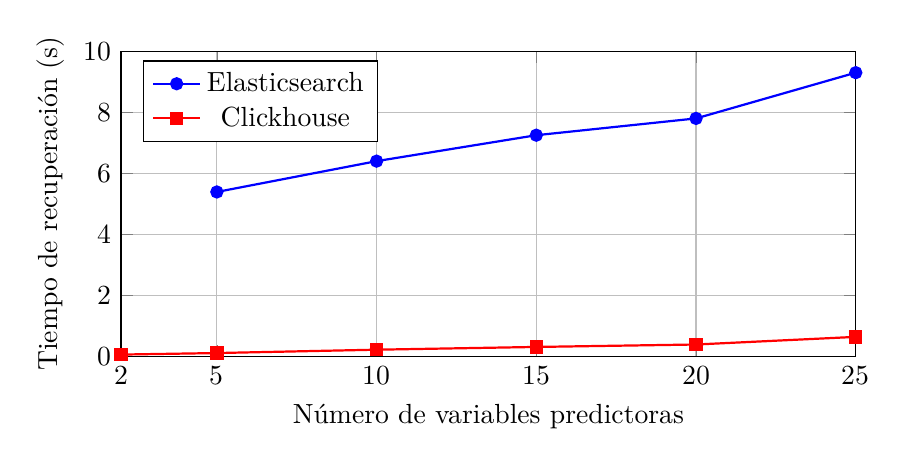
\begin{tikzpicture}
\begin{axis}[
  width=0.9\textwidth,
  height=0.45\textwidth,
  xlabel={Número de variables predictoras},
  ylabel={Tiempo de recuperación (s)},
  xmin=2, xmax=25,
  ymin=0, ymax=10,
  xtick={2,5,10,15,20,25},
  grid=major,
  legend pos=north west,
]
\addplot[
  color=blue,
  mark=*,
  thick
] coordinates {
  (5,5.39)
  (10,6.4)
  (15,7.25)
  (20,7.8)
  (25,9.3)
};
\addlegendentry{Elasticsearch}

\addplot[
  color=red,
  mark=square*,
  thick
] coordinates {
  (2,0.06)
  (5,0.11)
  (10,0.22)
  (15,0.31)
  (20,0.39)
  (25,0.64)
};
\addlegendentry{Clickhouse}
\end{axis}
\end{tikzpicture}
\caption{Gráfica de los tiempos de recuperación para la población Ensanut a partir de la última tabla.}
\label{fig:tiempos-ensanut}
\end{figure}

Esto nos muestra que Clickhouse es significativamente más rápido que Elasticsearch, incluso con un número pequeño de variables, 
esto se explica principalmente por su arquitectura orientada a columnas y su capacidad de paralelización, meintras que 
Elasticsearch, aunque es eficiente para búsquedas, no está optimizado para este tipo de consultas.

Por lo tanto, a partir de estos resultados, decidimos usar Clickhouse como nuestra herramienta para la recuperación de datos.

\subsection{5.2 Análisis de estabilidad.}\label{5.2-análisis-de-estabilidad-estadística.}

Parte importante de la validación empírica de un sistema es su estabilidad, en este caso queremos comprobar que la recuperación 
de datos es estable, es decir, que al hacer la misma consulta varias veces, el sistema tome tiempos similares.
Para esto, seleccionamos una consulta específica y la repetimos varias veces, obteniendo los siguientes resultados:

Para la población de Estudiantes, Académicos y Trabajadores de la UNAM, recuperamos los datos de 25 variables incluida 
la clase de interés, y obtuvimos los siguientes tiempos:


\begin{figure}[H]
\centering
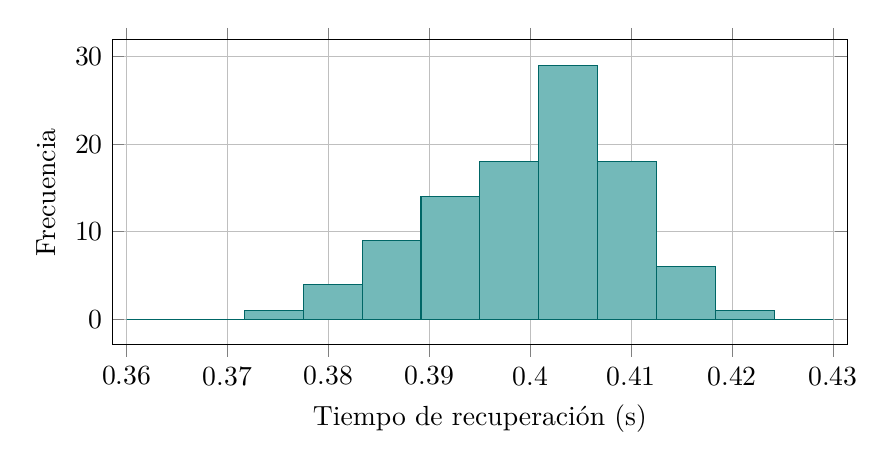
\begin{tikzpicture}
\begin{axis}[
  width=0.9\textwidth,
  height=0.45\textwidth,
  ybar,
  xlabel={Tiempo de recuperación (s)},
  ylabel={Frecuencia},
  xmin=0.36, xmax=0.43,
  grid=major,
  enlarge x limits=0.02,
]
\addplot+[
  hist={bins=12, data min=0.36, data max=0.43},
  fill=teal!55,
  draw=teal!80!black
] table[row sep=\\,y index=0] {
data\\
0.4053\\
0.4026\\
0.3845\\
0.4026\\
0.4140\\
0.3893\\
0.4094\\
0.3873\\
0.3918\\
0.4029\\
0.4107\\
0.4013\\
0.3897\\
0.4024\\
0.3937\\
0.4064\\
0.3936\\
0.4082\\
0.3819\\
0.3927\\
0.3808\\
0.4034\\
0.3952\\
0.4070\\
0.3993\\
0.4068\\
0.4187\\
0.3997\\
0.3965\\
0.4046\\
0.4064\\
0.3895\\
0.3855\\
0.4035\\
0.4151\\
0.4032\\
0.3960\\
0.4001\\
0.4053\\
0.4033\\
0.4107\\
0.4074\\
0.4007\\
0.4047\\
0.4069\\
0.3875\\
0.4063\\
0.4026\\
0.4071\\
0.3949\\
0.3913\\
0.4044\\
0.3925\\
0.4005\\
0.4029\\
0.4147\\
0.4038\\
0.3850\\
0.4013\\
0.3950\\
0.4099\\
0.3909\\
0.4049\\
0.4122\\
0.4018\\
0.3942\\
0.3975\\
0.4151\\
0.3871\\
0.3981\\
0.4091\\
0.4024\\
0.4076\\
0.4044\\
0.3964\\
0.4090\\
0.4019\\
0.3920\\
0.3969\\
0.3990\\
0.4131\\
0.4049\\
0.4099\\
0.3861\\
0.3959\\
0.4133\\
0.4003\\
0.3919\\
0.3757\\
0.4062\\
0.3833\\
0.3869\\
0.3855\\
0.4082\\
0.3987\\
0.4071\\
0.4049\\
0.3805\\
0.3987\\
0.4083\\
};
\end{axis}
\end{tikzpicture}
\caption{Histograma de 100 mediciones de tiempos de recuperación para la población de Estudiantes, Académicos y Trabajadores de la UNAM.}
\label{fig:histograma-unam-estabilidad}
\end{figure}



De manera similar, para la población de Ensanut recuperamos los datos de 25 variables incluida la clase de interés, y obtuvimos los siguientes tiempos:

\begin{figure}[H]
\centering
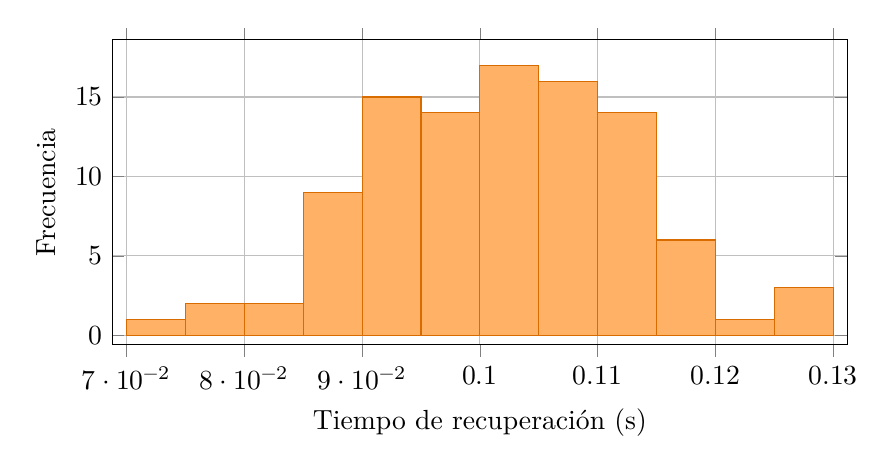
\begin{tikzpicture}
\begin{axis}[
  width=0.9\textwidth,
  height=0.45\textwidth,
  ybar,
  xlabel={Tiempo de recuperación (s)},
  ylabel={Frecuencia},
  xmin=0.07, xmax=0.13,
  grid=major,
  enlarge x limits=0.02,
]
\addplot+[
  hist={bins=12, data min=0.07, data max=0.13},
  fill=orange!60,
  draw=orange!85!black
] table[row sep=\\,y index=0] {
data\\
0.0915\\
0.0975\\
0.0920\\
0.0928\\
0.0964\\
0.1066\\
0.0968\\
0.1143\\
0.1189\\
0.0982\\
0.1111\\
0.1043\\
0.0912\\
0.0795\\
0.1123\\
0.0921\\
0.0871\\
0.1144\\
0.0956\\
0.1108\\
0.0933\\
0.1271\\
0.0804\\
0.1123\\
0.1053\\
0.0914\\
0.0994\\
0.0886\\
0.1062\\
0.1109\\
0.1131\\
0.1165\\
0.1170\\
0.0873\\
0.0898\\
0.0938\\
0.1118\\
0.1124\\
0.1008\\
0.0937\\
0.1090\\
0.1077\\
0.1111\\
0.0914\\
0.1025\\
0.1088\\
0.0815\\
0.0974\\
0.1181\\
0.1001\\
0.1272\\
0.0949\\
0.1028\\
0.0791\\
0.0877\\
0.1098\\
0.1150\\
0.0992\\
0.1096\\
0.1003\\
0.1016\\
0.0990\\
0.0877\\
0.1121\\
0.1123\\
0.1062\\
0.0931\\
0.0950\\
0.0918\\
0.1081\\
0.1000\\
0.0898\\
0.1076\\
0.1014\\
0.0976\\
0.1281\\
0.1002\\
0.1010\\
0.0866\\
0.0929\\
0.1007\\
0.0964\\
0.0973\\
0.1018\\
0.0874\\
0.1039\\
0.1115\\
0.1097\\
0.1051\\
0.1015\\
0.1061\\
0.1197\\
0.1065\\
0.1049\\
0.0984\\
0.1017\\
0.1210\\
0.0746\\
0.1097\\
0.0911\\
};
\end{axis}
\end{tikzpicture}
\caption{Histograma de 100 mediciones de tiempos de recuperación para la población de Ensanut.}
\label{fig:histograma-ensanut-estabilidad}
\end{figure}

Como podemos observar, en ambas poblaciones los tiempos de recuperación se encuentran bastante centradas alrededor de su media, 
lo cual nos da una buena indicación de que el sistema es estable.

\FloatBarrier



\subsection{5.3 Comparativa con la versión previa.}\label{5.3-comparativa-con-la-versión-previa.}


En esta sección queremos contrastar los tiempos totales de construcción de modelos entre la versión previa a la optimización y la 
versión aquí propuesta, para esto, consideraremos diferentes poblaciones así como diferentes cantidades de variables predictoras. 

Estas mediciones contemplan la construcción completa de los modelos, es decir, desde la recuperación de datos, pasando por la 
construcción de la estructura de datos S, la discretización de variables numéricas, el llenado del template con los conteos, así 
como el cálculo de epsilon y score, hasta la devolución de los resultados al frontend.

Con la población de Estudiantes, Académicos y Trabajadores de la UNAM, obtuvimos los siguientes tiempos totales 
de construcción de modelos:

\begin{table}[htbp]
\centering
\caption{Comparativa de tiempos totales de construcción de modelos entre versión previa y versión propuesta para la 
población de Estudiantes, Académicos y Trabajadores de la UNAM.}
\label{tab:comparativa-version-previa-propuesta}
\begin{tabular}{|l|c|c|c|c|c|}
\hline
Versión & 5 variables & 10 variables & 15 variables & 20 variables & 25 variables \\
\hline
Versión previa &5.57  &6.68  &7.56  &8.38  &10.1  \\
\hline
Versión propuesta &5.57  &6.68  &7.56  &8.38  &10.1  \\
\hline
\end{tabular}
\end{table}

Con la población de Ensanut, obtuvimos los siguientes tiempos totales de construcción de modelos:
\begin{table}[htbp]
\centering
\caption{Comparativa de tiempos totales de construcción de modelos entre versión previa y versión propuesta para la población de Ensanut.}
\label{tab:comparativa-version-previa-propuesta-ensanut}
\begin{tabular}{|l|c|c|c|c|c|}
\hline
Versión & 5 variables & 10 variables & 15 variables & 20 variables & 25 variables \\
\hline
Versión previa &5.57  &6.68  &7.56  &8.38  &10.1  \\
\hline
Versión propuesta &5.57  &6.68  &7.56  &8.38  &10.1  \\
\hline
\end{tabular}
\end{table}

Podemos observar que la versión propuesta es significativamente más rápida que la versión previa.



\section{Capítulo 6. Conclusiones}\label{capuxedtulo-6.-conclusiones}
Como conclusiones, se presentan algunos resultados interesantes que se obtuvieron a partir de la implementación del proyecto, 
así como algunas limitaciones que se encontraron durante el desarrollo del proyecto, y finalmente algunas ideas de optimización 
que se podrían implementar en un futuro para mejorar el rendimiento del sistema.

\subsection{6.1 Resultados principales.}
\subsection{6.2 Observaciones.}
\subsection{6.3 Limitaciones y trabajo futuro.}

Una de las limitantes del proyecto es que solamente se pueden crear modelos a partir 
de las poblaciones displonibles en la plataforma, esto se busca resolver en un futuro permitiendo que el usuario pueda 
subir sus propias poblaciones en algún formato en específico, y que la plataforma se encargue de procesar los datos y construir 
los modelos correspondientes.

Si bien el sistema propuesto es significativamente más rápido que la versión previa, aún hay margen de mejora, por ejemplo, 
buscar la manera de optimizar la discretización de variables numéricas, pues es la parte que del sistema que tiene la mayor 
complejidad temporal.
Aunque con las poblaciones y número de variables actuales el sistema es bastante rápido, si se quisiera usar con poblaciones más 
grandes, del orden de millones de observaciones, éste podría volverse lento.

\end{document}
